\subsection{Trigger system}

Trigger system in ATLAS is a very essential component, which is responsible for deciding whether to keep a given collision event for later study or not.
In LHC run-2, higher energy, luminosity and pile-up lead to an large increase of event rate by up to a factor of five, which cause to a even larger challenge and more strict requirement of trigger system.

The trigger system in run-2 is comprised of a hardware-based first level trigger (Level-1) and a software-based high level trigger (HLT) \cite{Ruiz-Martinez:2133909}.
As depicted in figure~\ref{fig:trig_syst}, in Level-1, the inputs from coarse granularity calorimeter and muon detector information together with some other subsystems are sent to the Central Trigger Processor to determine Regions-of-Interest (RoIs) in the detector. 
\begin{figure}[!htb]
  \centering
  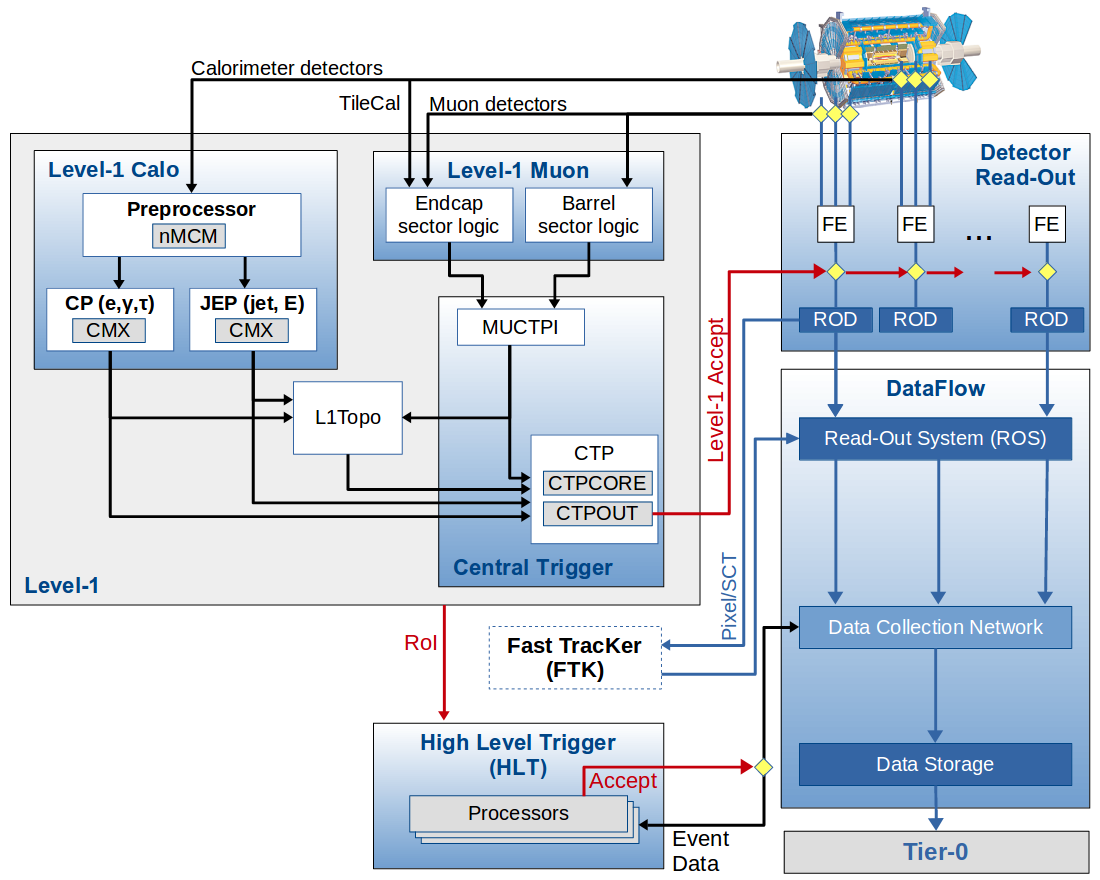
\includegraphics[width=0.9\textwidth]{figures/Detector/tdaq-run2-schematic2017.png}
  \caption{Schematic diagram of the ATLAS trigger and data acquisition system in Run-2.}
  \label{fig:trig_syst}
\end{figure}
The events rate can be reduced by Level-1 triggers from 30 MHz to 100 kHz. 
After that, the RoI information from Level-1 is sent to HLT, in which more sophisticated selection algorithms are run for regional reconstruction.
The HLT reduces the rate from Level-1 of 100 kHz to about 1 kHz on average.
At the end, the events that accepted by HLT are transfered to local storage at experimental site for offline reconstruction.
Details about Level-1 and HLT trigger systems will be described as belows.
